\documentclass{beamer}

\usepackage[orientation=landscape,size=a0,scale=1.4,debug]{beamerposter}
\mode<presentation>{\usetheme{mlr}}

\usepackage[sfdefault]{roboto}
\usepackage{roboto-mono}
\usepackage[T1]{fontenc}
\usepackage[utf8]{inputenc} % UTF-8
\usepackage[english]{babel} % Language
\usepackage{hyperref} % Hyperlinks
\usepackage{ragged2e} % Text position
\usepackage[export]{adjustbox} % Image position
\usepackage[most]{tcolorbox} % Code boxes

\hypersetup{
    hyperfootnotes=false,
    colorlinks=true,
	linktocpage=true,
	pdfauthor={mlr-org team},
    %linkcolor=[RGB]{3,99,142}, % mlr blue
    urlcolor=[RGB]{231,138,69}
}

\title{Dataflow programming with mlr3pipelines :\,: CHEAT SHEET} % Package title in header, \, adds thin space between ::

\newlength{\columnheight} % Adjust depending on header height
\setlength{\columnheight}{84cm}

\newtcolorbox{codebox}{%
	sharp corners,
	leftrule=0pt,
	rightrule=0pt,
	toprule=0pt,
	bottomrule=0pt,
	fontupper=\robotomono\small,
	hbox}

\newtcolorbox{codeboxmultiline}[1][]{%
	sharp corners,
	leftrule=0pt,
	rightrule=0pt,
	toprule=0pt,
	bottomrule=0pt,
	fontupper=\robotomono\small,
	#1}

\newtcolorbox{codeboxexample}{%
	sharp corners,
	leftrule=0pt,
	rightrule=0pt,
	toprule=0pt,
	bottomrule=0pt,
	fontupper=\robotomono\small,
	width=27cm,
	adjusted title=Example,
	fonttitle = \bfseries\Large,
	top = 0.5em}

\newtcolorbox{codeboxinline}{%
	sharp corners,
	leftrule=0pt,
	rightrule=0pt,
	toprule=0pt,
	bottomrule=0pt,
	hbox,
	nobeforeafter,
	fontupper=\robotomono\small,
	tcbox raise base}

\newcommand{\codeinline}[1]{\begin{codeboxinline}#1\end{codeboxinline}}
\newcommand{\monospace}[1]{\multido{}{#1}{\space}}

\begin{document}
\begin{frame}[fragile]{}
	\begin{columns}
		\begin{column}{.245\textwidth}
			\begin{beamercolorbox}[center]{postercolumn}
				\begin{minipage}{.98\textwidth}
					\parbox[t][\columnheight]{\textwidth}{
						\begin{myblock}{Intro}
              Combine ML operations to flexible pipelines and processing graphs, which can be configured trained, resampled, tuned as any regular learner.
              % The mlr3pipelines package is an extension for the \href{https://github.com/mlr-org/mlr3}{mlr3} package and provides \codeinline{PipeOp}s (pipeline operators) which can be connected to a \codeinline{Graph} using, e.g., the \%>{}>\% operator.
            \end{myblock}
						\begin{myblock}{PipeOps}
              Flow operation with train and predict step. During train, transforms input and learns a state. During predict, applies transforms input with stored state.
              \begin{center}
                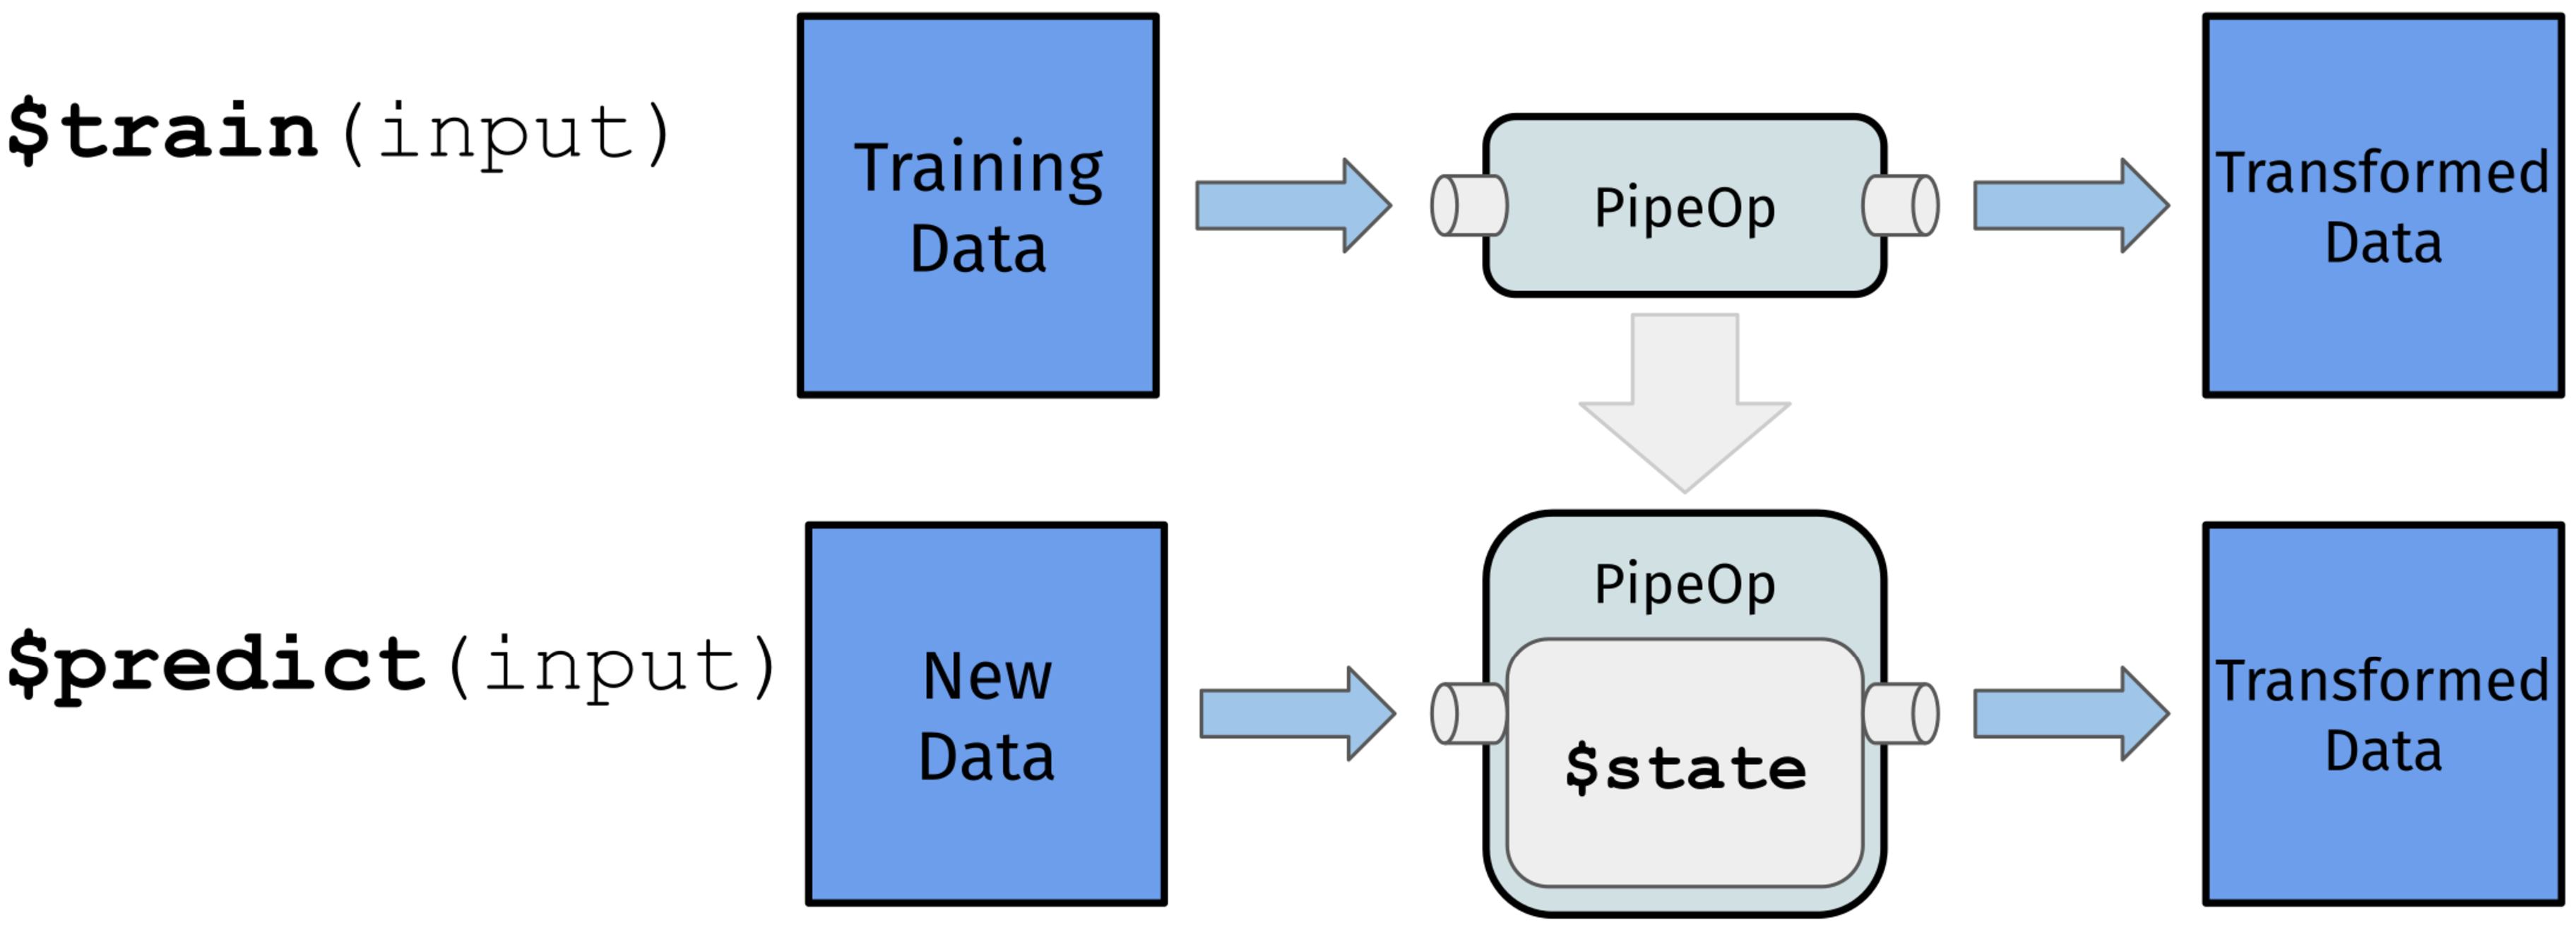
\includegraphics[width=0.7\textwidth]{img/po.pdf}
              \end{center}
              \ \\
              Construction via a \codeinline{key}, e.g.: \codeinline{pca = \textbf{po}("pca")} \\
              \ \\
              Important methods and slots:
              \begin{itemize}
                \item \codeinline{\textbf{\$train}(input)}: arg is named list
                \item \codeinline{\textbf{\$predict}(input)}: arg is named list
                \item \codeinline{\textbf{\$state}} 
                % obtained during training and usually required for prediction
                \item \codeinline{\textbf{\$param\_set}} see Hyperparameters
              \end{itemize}
  			\end{myblock}
            \begin{myblock}{Important PipeOps}
              \begin{footnotesize}
                \begin{centering}
                  \begin{tabular}{l l l}
                    \textbf{Class} & \textbf{Key} & \textbf{Operation} \\ \hline
                    PipeOpPCA & "pca" & Data Transformer\\
                    PipeOpFilter & "filter" & Feature Selection\\
                    PipeOpRemoveConstants & "removeconstants" & Repair Tasks\\
                    PipeOpEncode & "encode" & Factor Encoding\\
                    PipeOpClassBalancing & "classbalancing" & Imbalanced Data\\
                    PipeOpImputeMean & "imputemean" & Missing Data\\
                    PipeOpLearner & "learner" & Any Learner\\
                    PipeOpLearnerCV & "learner\_cv" & Ensembles\\
                    PipeOpMutate & "mutate" & Fearure Engineering\\ \hline
                  \end{tabular}
                \end{centering}
              \end{footnotesize}
              \ \\
              \ \\
              \ \\
              Full list: \codeinline{as.data.table(mlr\_pipeops)}
						\end{myblock}
						\vfill}
				\end{minipage}
			\end{beamercolorbox}
		\end{column}
		\begin{column}{.245\textwidth}
			\begin{beamercolorbox}[center]{postercolumn}
				\begin{minipage}{.98\textwidth}
					\parbox[t][\columnheight]{\textwidth}{
						\begin{myblock}{Graphs}
              Connects \codeinline{PipeOp}s with edges to control data flow during training and prediction. Input is sent to sources (no incoming edges), output is read from sinks (no outoing edges) of the graph. \codeinline{PipeOp}s can have different numbers of \codeinline{\$input}s and  \codeinline{\$output}s.\\
              % The return value corresponds to the output of the \codeinline{PipeOp} outputs that are not connected to other \codeinline{PipeOp}s.\\
              % Trained and predicted \codeinline{Graph} has a \codeinline{\$train()} and \codeinline{\$predict()} method that accept data and propagate this data through the network of \codeinline{PipeOp}s. The return value corresponds to the output of the \codeinline{PipeOp} outputs that are not connected to other \codeinline{PipeOp}s.\\
              \ \\
              The \codeinline{\%>{}>\%} operator takes either a \codeinline{PipeOp} or a \codeinline{Graph} on each of its sides and connects all left-hand outputs to the right-hand inputs; this requires the number of outputs and inputs to match:
              \begin{codebox}
                gr = po("pca") \textbf{\%>{}>\%} lrn("classif.rpart")
              \end{codebox}
              \ \\
              For full control of input-output connection, construct an empty \codeinline{Graph}, add \codeinline{PipeOp}s and connect them via their \codeinline{\$id}:
              \begin{codeboxmultiline}[width=23cm]
                gr = \textbf{Graph}\$new()\\
                gr\$\textbf{add\_pipeop}(po("pca"))\\
                gr\$\textbf{add\_pipeop}(lrn("classif.rpart"))\\
                gr\$\textbf{add\_edge}("pca", "classif.rpart")
              \end{codeboxmultiline}
              \leavevmode
              \begin{itemize}
                \item Printing: \codeinline{\textbf{print}(gr)}\\
                \item Plotting: \codeinline{gr\$\textbf{plot}(html = TRUE)}\\
                \item Assessing the \codeinline{PipeOp}s: \codeinline{gr\$\textbf{pipeops}}
              \end{itemize}
              \ \\
              A \codeinline{GraphLearner} can be constructed from any \codeinline{Graph} and behaves like any other \codeinline{Learner}: \codeinline{grl = \textbf{GraphLearner}\$new(gr)}\\
              \ \\
              See the slots \codeinline{\$encapsulate} for debugging and \codeinline{\$model} for results after training. Predicting probabilities requires to set the predict type explicitly \codeinline{grl\$predict\_type = "prob"}.
						\end{myblock}
						\vfill}
				\end{minipage}
			\end{beamercolorbox}
		\end{column}
		\begin{column}{.245\textwidth}
			\begin{beamercolorbox}[center]{postercolumn}
				\begin{minipage}{.98\textwidth}
					\parbox[t][\columnheight]{\textwidth}{
            \begin{myblock}{Linear Graphs}
              The main purpose of a \codeinline{Graph} is to build combined preprocessing and model fitting pipelines that can be used as a \codeinline{Learner}. Often, a \codeinline{Graph} (or a \codeinline{GraphLearner}) resembles a linear structure and only requires use of \%>{}>\%. The following schematic shows a \codeinline{GraphLearner} centering and scaling features, encoding factors and imputing missing data before a \codeinline{Learner} is applied.
              \begin{center}
                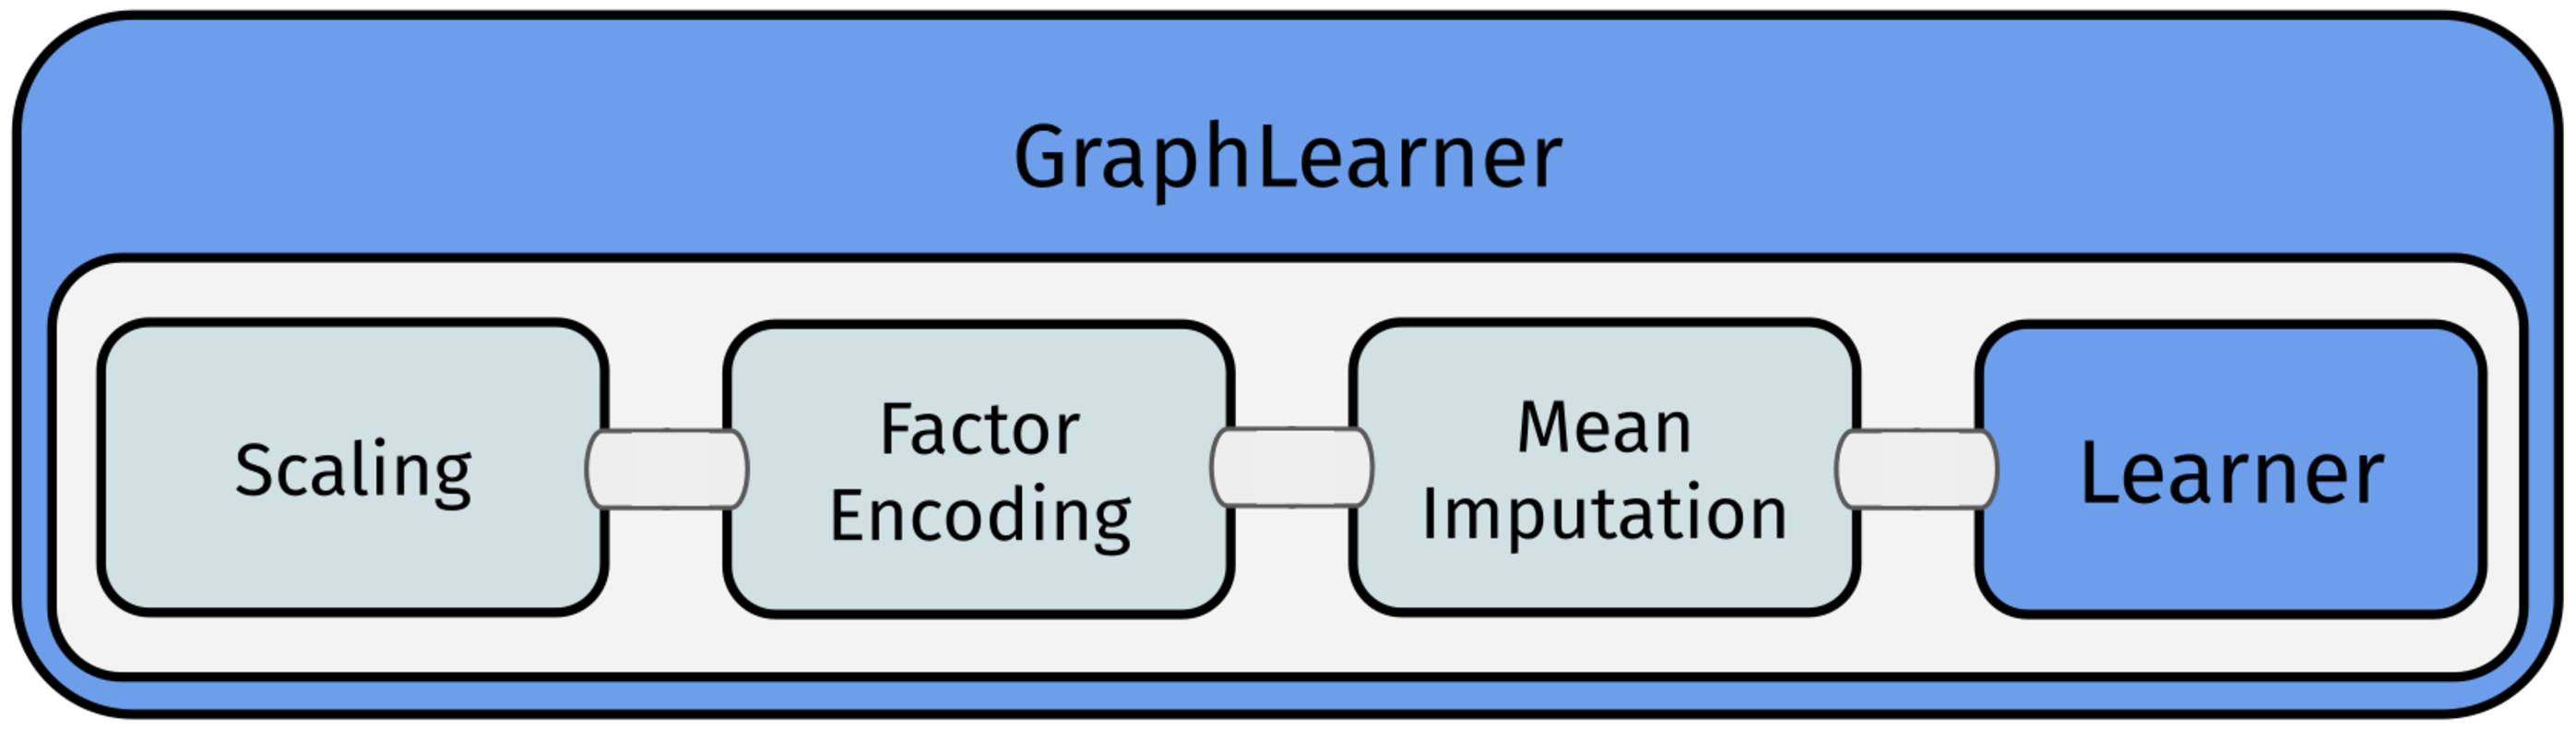
\includegraphics[width=0.7\textwidth]{img/grl_linear.pdf}
              \end{center}
              \ \\
              \begin{codeboxexample}
                {\footnotesize
                  \# construct the graph learner:\\
                  grl = GraphLearner\$new(po("scale") \%>{}>\%\\
                  \hspace*{1ex} po("encode") \%>{}>\% po("imputemean") \%>{}>\%\\
                  \hspace*{1ex} lrn("classif.rpart"))\\
                  \ \\
                  \# train on a task:\\
                  grl\$train(task)\\
                  \# and look at the results:\\
                  grl\$model\\
                  \ \\
                  \# predict on a (new) task:\\
                  grl\$predict(task)\\
                  \ \\
                  \# perform resampling (3-fold cv):\\
                  rcv = rsmp("cv", folds = 3)\\
                  rcv\$instantiate(task)\\
                  rr = resample(task, grl, rcv)}
              \end{codeboxexample}
            \end{myblock}
				    \vfill}
				\end{minipage}
			\end{beamercolorbox}
		\end{column}
    \begin{column}{.245\textwidth}
			\begin{beamercolorbox}[center]{postercolumn}
				\begin{minipage}{.98\textwidth}
					\parbox[t][\columnheight]{\textwidth}{
             \begin{myblock}{Nonlinear Graphs}
              Multiple input or output channels allow for nonlinear \codeinline{Graphs}. Useful functions in this context are \codeinline{gunion()} and \codeinline{greplicate()}.\\
              \ \\
              \codeinline{\textbf{gunion}()} arranges \codeinline{PipeOp}s or \codeinline{Graph}s next to each other in a disjoint graph union.
              \begin{center}
                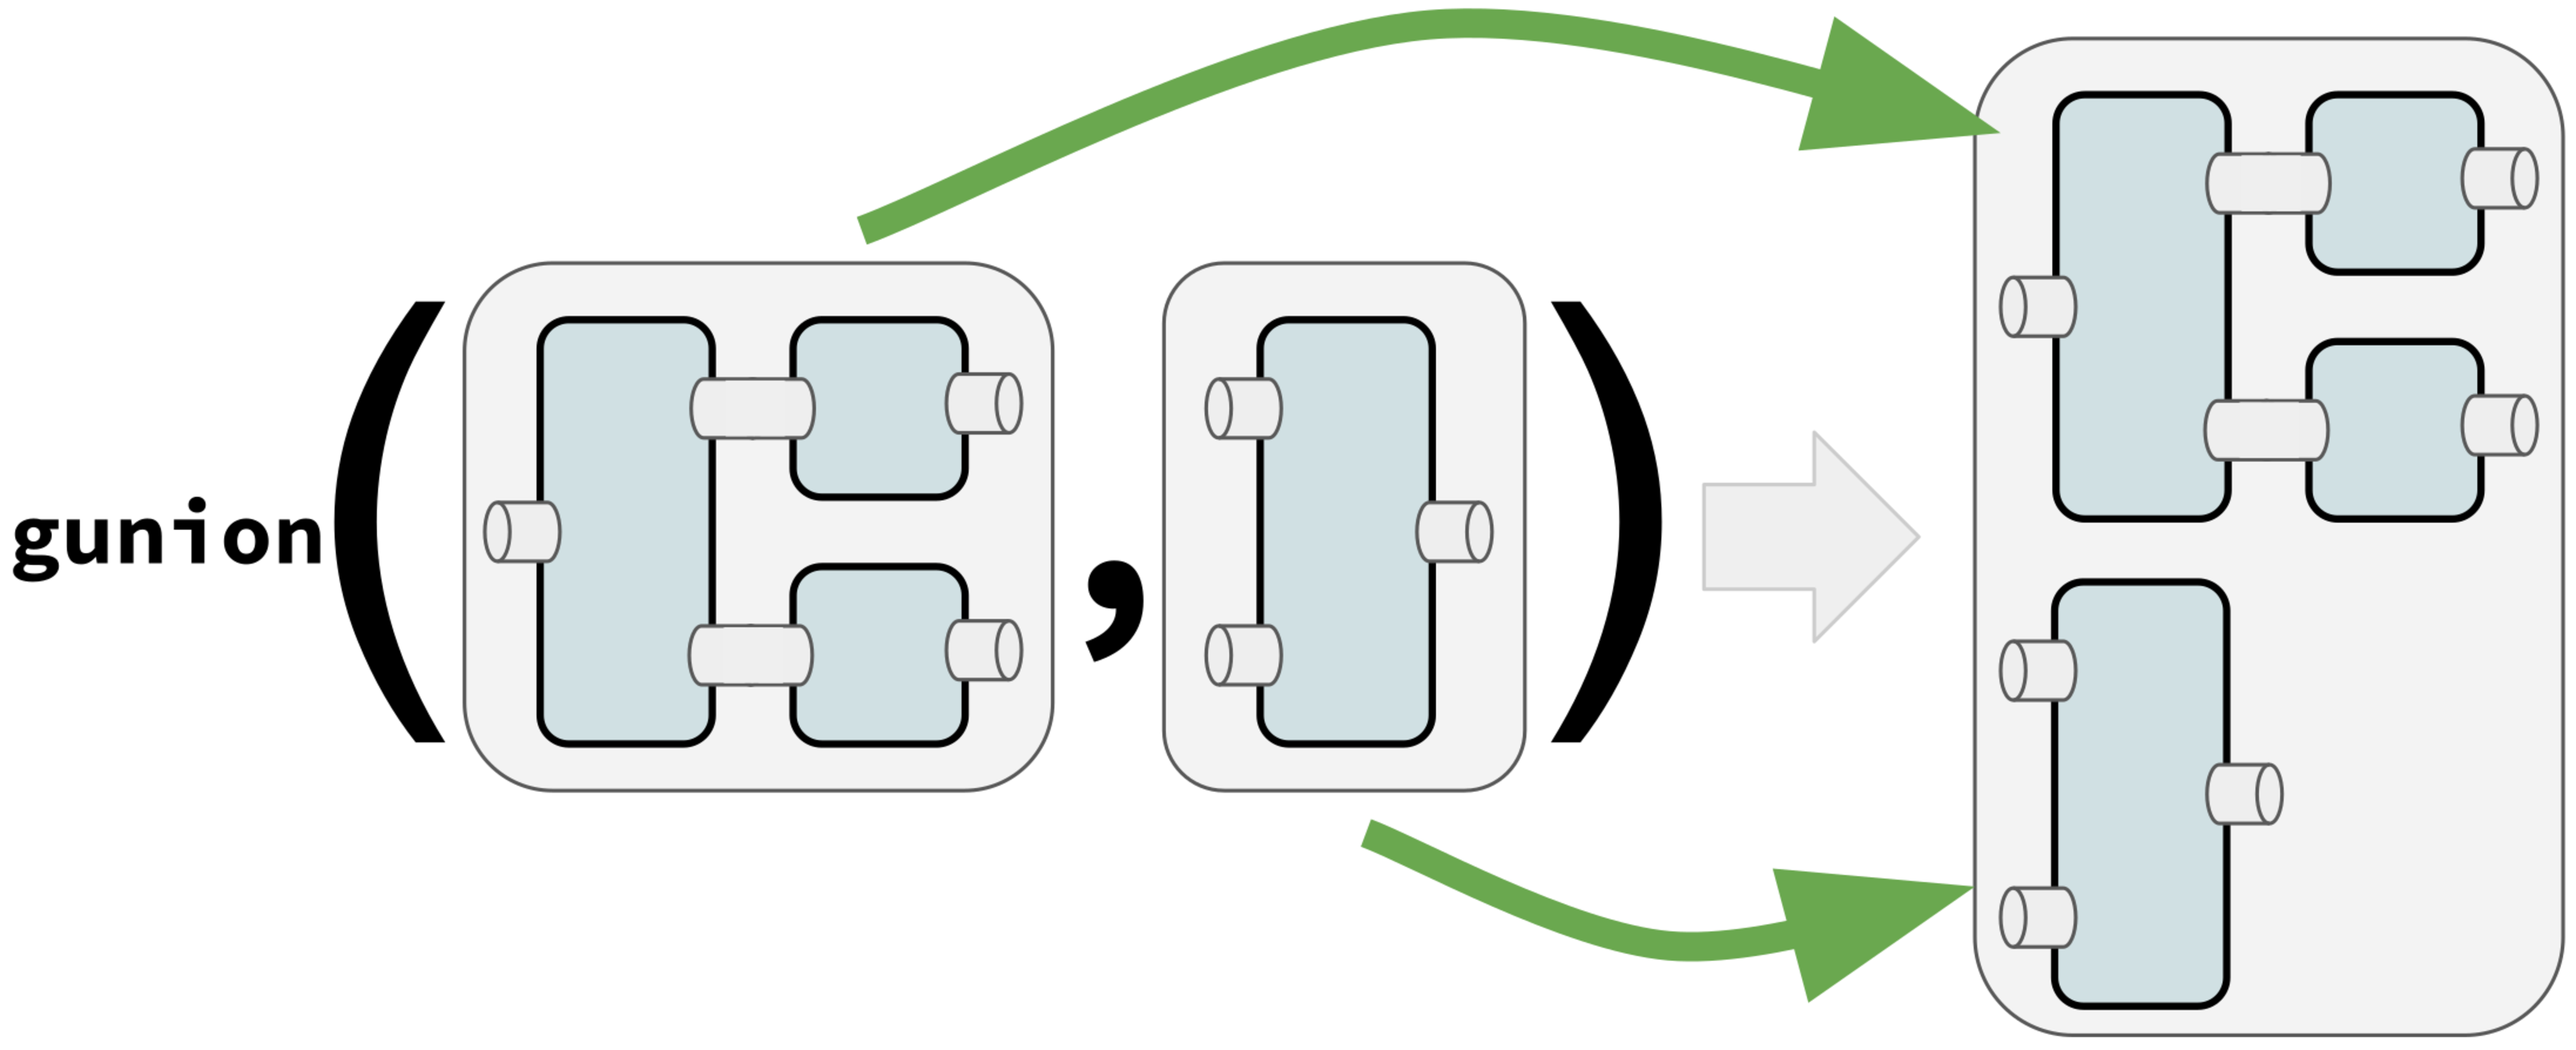
\includegraphics[width=0.7\textwidth]{img/gunion.pdf}
              \end{center}
              Using \codeinline{PipeOpBranch} and \codeinline{PipeOpUnbranch}, this allows for splitting a node into several paths, called \textbf{branching} (in the following, only one path, pca or scale, can be set active at a time):
              \begin{codeboxexample}
						    {\footnotesize
                  \# embed pca and scale between branch and unbranch:\\
                  choices = c("pca", "scale")\\
                  gr = po("branch", options = choices) \%>{}>\%\\
                  \hspace*{1ex} gunion(list(po("pca"), po("scale"))) \%>{}>\%\\
                  \hspace*{1ex} po("unbranch", options = choices)\\
                  \# set the pca path active:\\
                  \ \\
                  gr\$param\_set\$values\$branch.selection = "pca"}
					      \end{codeboxexample}
              \ \\
              \codeinline{\textbf{greplicate}()} creates a new \codeinline{Graph} containing \codeinline{n} copies of the input (\codeinline{PipeOp} or \codeinline{Graph}).
              \begin{center}
                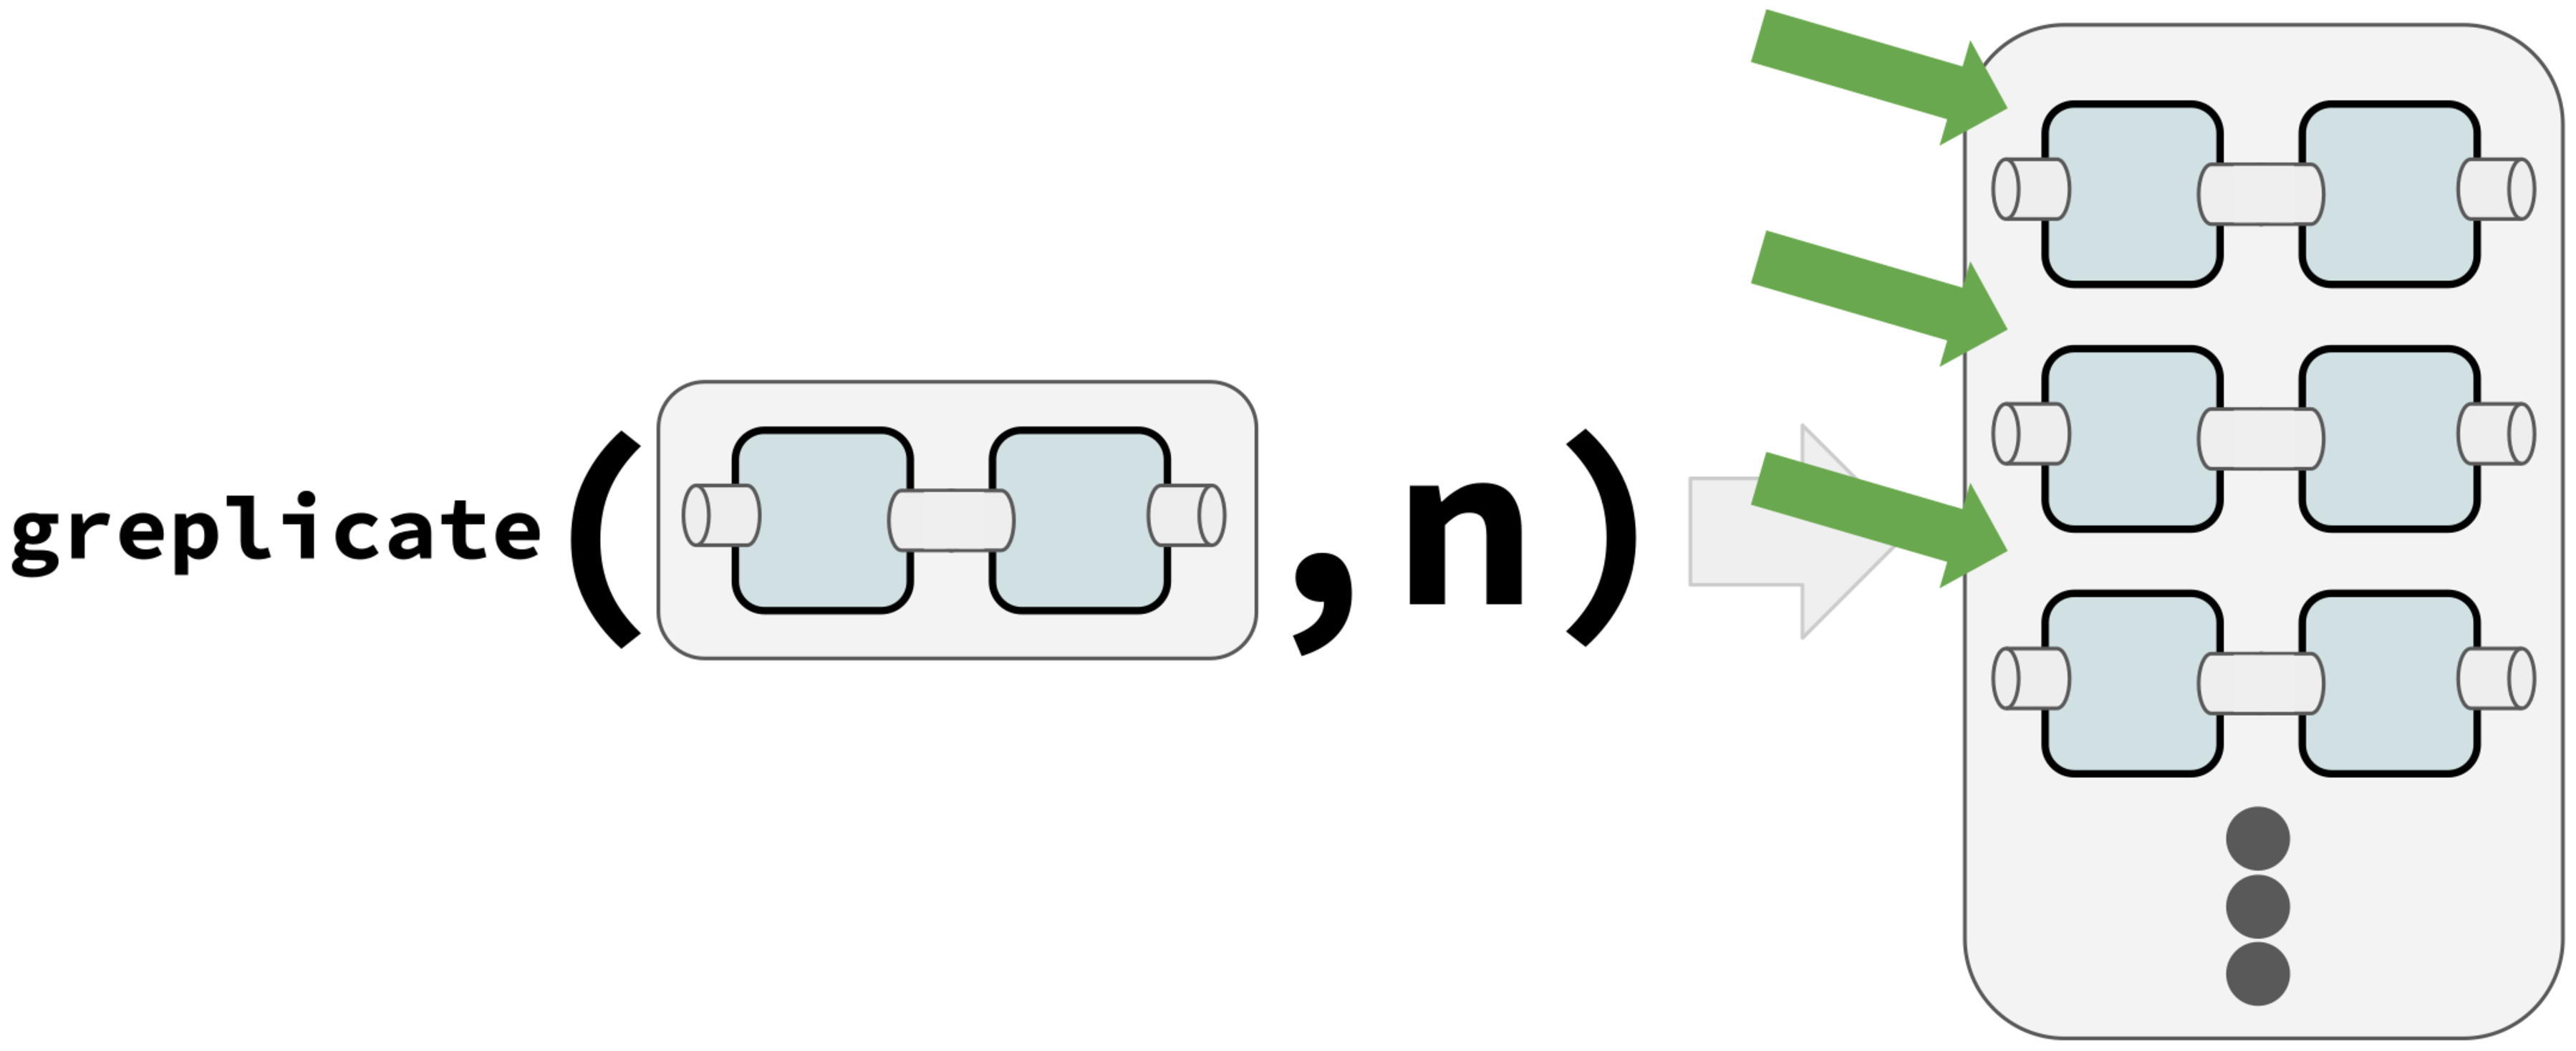
\includegraphics[width=0.7\textwidth]{img/greplicate.pdf}
              \end{center}
              Together with \codeinline{PipeOpSubsample} this straightforward allows for, e.g., \textbf{bagging} (subsampling, refitting and averaging):
              \begin{codeboxexample}
						    {\footnotesize
                  \# simple subsample and learner\\
                  pr = po("subsample") \%>{}>\% lrn("classif.rpart")\\
                  \# 10 replicates with averaging over predictions\\
                  bagging = greplicate(pr, n = 10) \%>{}>\%\\
                  \hspace*{1ex} po("classifavg", innum = 10)}
					    \end{codeboxexample}
            \end{myblock}
            \vfill}
         \end{minipage}
	    \end{beamercolorbox}
		\end{column}
 \end{columns}
\end{frame}
\begin{frame}[fragile]{}
	\begin{columns}
		\begin{column}{.245\textwidth}
			\begin{beamercolorbox}[center]{postercolumn}
				\begin{minipage}{.98\textwidth}
					\parbox[t][\columnheight]{\textwidth}{
            \codeinline{PipeOpFeatureUnion} aggregates features from all input tasks into a single \codeinline{Task} (in the example below, we combine the original features obtained from \codeinline{PipeOpNOP} with the principal components obtained from the pca):
              \begin{codeboxexample}
						    {\footnotesize
                  \# copy input to nop and pca; combine the features:\\
                  gr = po("copy", outnum = 2) \%>{}>\%\\
                  \hspace*{1ex} gunion(list(po("nop"), po("pca"))) \%>{}>\%\\
                  \hspace*{1ex} po("featureunion")}
              \end{codeboxexample}
              \begin{myblock}{Special PipeOps}
                \codeinline{PipeOpImpute} imputes missing data. Methods include e.g. mean, median and histogram imputation.\\
                \ \\
                \codeinline{PipeOpMutate} allows for adding new features. This works by providing expressions in an \codeinline{alist}:
                \begin{codeboxexample}
                  \footnotesize{
                  task = tsk("iris")\\
                  \# add new features related to the iris task:\\
                  mutations = list(\\
                  \hspace*{1ex} Sepal.Sum = \char`\~ \ Sepal.Length + Sepal.Width,\\
                  \hspace*{1ex} Petal.Sum = \char`\~ \ Petal.Length + Petal.Width\\
                  )\\
                  mutate = po("mutate", param\_vals =\\
                  GraphLearner\$new(mutate \%>{}>\% lrn("classif.rpart"))
                  \hspace*{1ex} list(mutation = mutations))}
                \end{codeboxexample}
                \ \\
                \codeinline{PipeOpChunk} allows for splitting data into several parts.\\
                \ \\
                \codeinline{PipeOpFilter} can be used with filters from the mlr3filters package. Use this so select features for subsequent learners.\\
                \ \\
                \codeinline{PipeOpSelect} removes features from a task given a \codeinline{Selector} function defining the features to keep.
              \end{myblock}
           	\vfill}
				\end{minipage}
			\end{beamercolorbox}
		\end{column}
    \begin{column}{.245\textwidth}
			\begin{beamercolorbox}[center]{postercolumn}
				\begin{minipage}{.98\textwidth}
					\parbox[t][\columnheight]{\textwidth}{
            \begin{myblock}{Hyperparameters}
              % mlr3pipelines relies on the paradox package to provide parameters that can modify a \codeinline{PipeOp}'s or \codeinline{Graph}'s behavior. 
              To inspect the parameters see the \codeinline{\$param\_set}, e.g., \codeinline{po("pca")\$\textbf{param\_set}}.\\
              \ \\
              Access the \codeinline{\$param\_set\$values} slot to set or retrieve a parameter, or specify \codeinline{param\_vals} during construction:
              \begin{codeboxmultiline}[width=24cm]
                {\footnotesize pca = po("pca") \\
                pca\$param\_set\$\textbf{values} = list(scale. = TRUE) \\
                \# alternatively:\\
                po("pca", \textbf{param\_vals} = list(scale. = TRUE))}
              \end{codeboxmultiline}
              \ \\
              In a \codeinline{Graph}, the parameters of all \codeinline{PipeOp}s are collected. A \codeinline{GraphLearner} preserves the parameters of its encapsulated objects.
            \end{myblock}
            \begin{myblock}{Tuning}
              Done as with any other \codeinline{Learner} (see \href{FIXME:CheatsheetLink}{mlr3tuning}). E.g., use an \codeinline{AutoTuner} for the rank parameter of the PCA and the complexity parameter of rpart with respect to the classification error as the performance measure:
              \begin{codeboxexample}
						  {\footnotesize
                task = tsk("iris")\\
                \# pca and rpart as GraphLearner:\\
                gr = po("pca") \%>{}>\% lrn("classif.rpart")\\
                grl = GraphLearner\$new(gr)\\
                \ \\
                \# inner loop holdout:\\
                resampling\_inner = rsmp("holdout")\\
                measures = msr("classif.ce")\\
                \# define the tuning parameters:\\
                tune\_ps = ParamSet\$new(list(\\
                \hspace*{1ex} ParamInt\$new("pca.rank.", lower = 1, upper = 4),\\
                \hspace*{1ex} ParamDbl\$new("classif.rpart.cp",\\
                \hspace*{2ex} lower = 0, upper = 0.05)\\
                ))\\
                \# 20 evaluations using grid\_search:\\
                terminator = term("evals", n\_evals = 20)\\
                tuner = tnr("grid\_search", resolution = 5)\\
                \ \\
                \# set up the auto tuner:\\
                at = AutoTuner\$new(grl, resampling\_inner,\\
                \hspace*{1ex} measures, tune\_ps, terminator, tuner)\\
                \ \\
                \# outer loop 2-fold cv:\\
                resampling\_outer = rsmp("cv", folds = 2)\\
                \ \\
                rr = resample(task, at, resampling\_outer)}
					    \end{codeboxexample}
            \end{myblock}
						\vfill}
        \end{minipage}
			\end{beamercolorbox}
		\end{column}
    \begin{column}{.245\textwidth}
			\begin{beamercolorbox}[center]{postercolumn}
				\begin{minipage}{.98\textwidth}
					\parbox[t][\columnheight]{\textwidth}{
            \begin{myblock}{}
            \end{myblock}
						\vfill}
        \end{minipage}
			\end{beamercolorbox}
		\end{column}
    \begin{column}{.245\textwidth}
			\begin{beamercolorbox}[center]{postercolumn}
				\begin{minipage}{.98\textwidth}
					\parbox[t][\columnheight]{\textwidth}{
            \begin{myblock}{}
            \end{myblock}
						\vfill}
        \end{minipage}
			\end{beamercolorbox}
		\end{column}
	\end{columns}
\end{frame}
\end{document}
